% TODO
Insgesamt wurden 29 Unit-Test geschrieben. Im Folgenden werden auf Einzelheiten zu den Unit-Tests eingegangen.
\subsection{ATRIP}
Die entwickelten Unit-Tests befolgen die ATRIP-Regeln.
Das bedeutet also, dass sie...
\begin{itemize}
\item Automatic, also eigenständig ablaufen und ihre Ergebnisse selbst prüfen.
\item Thorough, also gründlich (genug) sind und die wichtigsten Funktionalitäten prüfen. Dazu gehört bei unserem Use-Case:
\begin{itemize}
\item Die Analyse der Wetterdaten,
\item Die Validierung der vom Nutzer eingegebenen Konfiguration,
\item Das Decodieren der Konfiguration,
\item Die Verarbeitung der Daten der APIs, sowie die Fehlerbehandlung der APIs
\end{itemize}
\item Repeatable, also jederzeit (automatisch) ausführbar sind. Dabei wird beispielsweise im Falle des WeatherInterpreterTest darauf geachtet, dass der Test nicht von der aktuellen Systemzeit abhängig ist.
\item Independent, also unabhängig voneinander in beliebiger Reihenfolge ausführbar sind. Kein Test ist auf das Ergebnis oder den Ablauf eines anderen Tests abhängig.
\item Professional, also einfach verständlich sind.
\end{itemize}
Hier wahrscheinlich noch Screenshots für die einzelnen Unterpunkte
\subsection{Beispiel für Unit-Tests und Mocks}
Die Unit-Test wurden, sofern möglich, in der AAA-Normalform entwickelt. Bei Unit-Tests, die Exceptions erwarten musste der Act- und Assert-Schritt teilweise zusammengeführt werden. In Listing \ref{ConfValidator} wird einerseits gezeigt, wie der zu testende ConfigValidator im Konstruktor vor jedem Testdurchlauf neu initialisiert wird und die \texttt{ValidationAspects} registriert werden. Im Test selbst wird eine fehlerhafte Konfiguration erzeugt, da im Stadtnamen Zahlen vorhanden sind. Daraufhin wird überprüft, ob die Validierung die richtige \texttt{Exception} wirft und ob die \texttt{ExceptionMessage} richtig ist, also der Fehler korrekt erkannt wurde.

\begin{listing}[h]
\inputminted[linenos=true,frame=lines]{csharp}{Listings/ConfigValidatorTest.cs}
\caption{Unit-Test für den ConfigValidator}
\label{ConfValidator}
\end{listing}

Als Beispiel für Mocks betrachten wir in Listing \ref{ImageHandler} ein Test für den \texttt{ImageHandler}. Dabei wird das Interface \texttt{IAPICaller} gemockt und die in Zeile x definierte \texttt{correctApiResponse} beim Aufruf der \texttt{Get}-Methode des API-Callers zurückgegeben. Durch den Einsatz des Mocks, lässt sich die Funktionalität des \texttt{ImageHandlers} testen ohne einen realen API-Caller zu verwenden. Am Schluss wird überprüft, ob das Ergebnis des Aufrufs mit dem erwarteten, eingegebenen Ergebnis übereinstimmt.

\begin{listing}[h]
\inputminted[linenos=true,frame=lines]{csharp}{Listings/ImageHandlerTest.cs}
\caption{Unit-Test für den ImageHandler mit Mock}
\label{ImageHandler}
\end{listing}

\subsection{Code Coverage}
Mithilfe der Visual Studio 2019 Enterprise Version lässt sich die Code Coverage für das Projekt ermitteln. Dabei erreicht WeatherWallpaper eine Code Coverage von knapp 42\%. Dies ist in Abbildung \ref{CodeCoverage} zu sehen. 
\begin{figure}[ht]
\centering
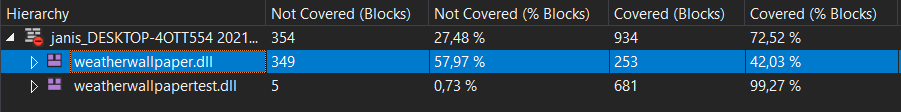
\includegraphics[width=\textwidth]{Bilder/CodeCoverage}
\caption[Code Coverage Ergebnisse]{\label{CodeCoverage} Code Coverage Ergebnisse}
\end{figure}
Des Weiteren bietet das Visual Studio Tool die Möglichkeit einzusehen, welche Zeilen von den Tests abgedeckt werden und welche nicht. Zeilen die nicht abgedeckt werden, werden rot hinterlegt und abgedeckte Zeilen blau, wie in Abbildung \ref{CodeCoverageHighlight} zu sehen.
\begin{figure}[ht]
\centering
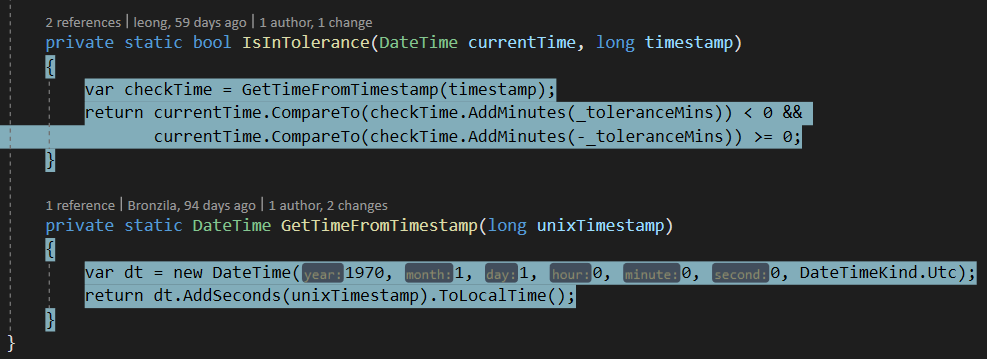
\includegraphics[width=\textwidth]{Bilder/CodeCoverageHighlighted}
\caption[Code Coverage Ergebnisse]{\label{CodeCoverageHighlight} Code Coverage Highlighting}
\end{figure}